\chapter{Description of tasks}
Before starting, I would like to thank my dear friend Alex Herrero to share with me his Latex project that he did for GEP months ago \cite{herrero_facultat_nodate}.
I will use his Gantt chart as template for mine, so I will not need to spend time in the creation and investigation of pgfgantt package. \\

This project officially started the second week of February 2024 although some mails and meets were done before with supervisor and co-supervisor.
I will not include this previous work in the planning, as I consider not necessary.
This work will be done during the following months, until the third week of June 2024, approximately one week before the oral defense.
This is a total of 17 weeks and TFG is an 18 ECTS project, so it will need 450 hours of work, 26 hours per week approximately.
Here I will define the principal sections of my project, with the possible resources needed and the minimum hours needed:

\section{Project definition and planning \textbf{(G)} }
This section includes everything done in GEP, since its completion is mandatory and has set deadlines.
So, all the following task are documentation and only requires my personal laptop since I have the entire environment required to develop in \LaTeX.
I also may need to contact my supervisor to check some details and ask for some doubts and also check for my GEP tutor feedback of every deliverable.
This task has a linear dependency (\textbf{see Figure \ref{G_dependences}}) because of GEP structure (in reality the only dependence is that G4 needs to be done the last one).
\begin{itemize}
    \item \textbf{G1} Context and Scope \\
        This corresponds to the first deliverable of GEP, where is defined the context and scope of the project. \\
        Role: Project Manajer \\
        Expected dedication: 20 hours
    \item \textbf{G2} Planning \\
        This corresponds to the second deliverable of GEP, where is defined the planning of the project. \\
        Role: Project Manajer \\
        Expected dedication: 12 hours
    \item \textbf{G3} Budget and Sustainability \\
        This corresponds to the third deliverable of GEP, where is defined the budged and sustainability of the project. \\
        Role: Project Manager \\
        Expected dedication: 18 hours 
    \item \textbf{G4} Final Document \\
        This corresponds to the last deliverable of GEP, where contains all the previous deliverables together with the necessary improvements using the feedback. \\
        Role: Project Manajer \\
        Expected dedication: 25 hours
\end{itemize}
\begin{figure}[h]
    \centering
    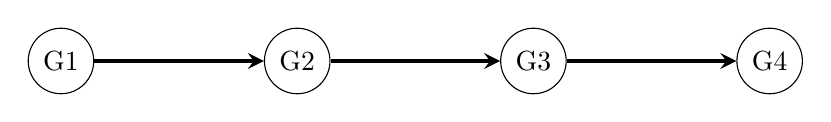
\begin{tikzpicture}
      % Define nodes
      \node[circle, draw] (A) at (0,0) {G1};
      \node[circle, draw] (B) at (3,0) {G2};
      \node[circle, draw] (C) at (6,0) {G3};
      \node[circle, draw] (D) at (9,0) {G4};
      
      % Define edges
      \draw[->, >=stealth, line width=1.5pt] (A) -- (B);
      \draw[->, >=stealth, line width=1.5pt] (B) -- (C);
      \draw[->, >=stealth, line width=1.5pt] (C) -- (D);
    \end{tikzpicture}
    \caption{Task Dependencies for Project definition and planning, self elaborated}
    \label{G_dependences}
\end{figure}

\section{Research and Learning \textbf{(RL)}}
In this section is included all the research and learning that I need for the correct development of the project.
Here I will only need access to internet to search for information and access to the different pages and documents that I will be using.
The principal internet resources that I will use are: Juan Pablo's TFM \cite{TFM}, Haskell notes made by Jordi Petit from the subject LP \cite{ApuntesHaskell} and the Dynamic Pipeline Framework repository \cite{GitHubDynamicPipeline}.
I may also need to contact my supervisor for Haskell doubts and also Juan Pablo if some critical doubt appears.
This section also have some dependence (\textbf{see Figure \ref{RL_dependences}}) because of the nature of the tasks.
\begin{itemize}
    \item \textbf{RL1} Haskell Refresh \\
        The refresh of my Haskell knowledge and improvement of it. 
        Check for possible libraries and codes \\
        Role: Project Manajer \\
        Expected dedication: 20 hours
    \item \textbf{RL2} TFM assimilation\\
        The reading and understanding of Juan Pablo's work. \\
        Role: Researcher \\
        Expected dedication: 25 hours
    \item \textbf{RL3} Dynamic Pipeline Framework \\
        Intensive review of the framework repository. \\
        Role: Haskell Developer \\
        Expected dedication: 30 hours 
\end{itemize}
\begin{figure}[h]
    \centering
    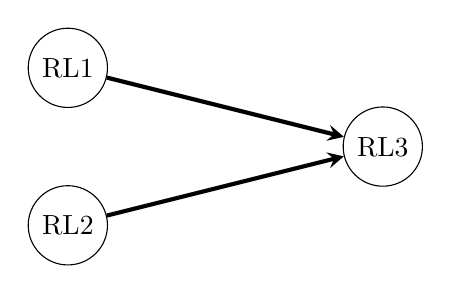
\begin{tikzpicture}
      % Define nodes
      \node[circle, draw] (A) at (0,2) {RL1};
      \node[circle, draw] (B) at (0,0) {RL2};
      \node[circle, draw] (C) at (4,1) {RL3};
      
      % Define edges
      \draw[->, >=stealth, line width=1.5pt] (A) -- (C);
      \draw[->, >=stealth, line width=1.5pt] (B) -- (C);
    \end{tikzpicture}
    \caption{Task Dependencies for Research and Learning, self elaborated}
    \label{RL_dependences}
\end{figure}

\section{First Algorithm Development \textbf{(FA)}}
This section includes the development of the first algorithm, the one that will be put to test my Haskell knowledge acquired.
Here I will need my personal laptop (as I have the entire environment required) and access to the GitHub repository \cite{GitHubTFG}.
For all the Haskell doubts I may need to contact my supervisor and for Dynamic pipeline doubts I should contact my co-supervisor as she is the expert.
This task has a linear dependency (\textbf{see Figure \ref{FA_dependences}}), but a critical testing error may need to reimplement some parts of the code, generating a circular dependency.
\begin{itemize}
    \item \textbf{FA1} Algorithm Scaffold \\
        Here will be set the base of the algorithm and the form of the dynamic pipeline.
        Check for possible libraries and codes \\
        Role: Haskell Developer\\
        Expected dedication: 20 hours
    \item \textbf{FA2} Algorithm Implementation\\
        This part is the pure implementation of the algorithm. \\
        Role: Haskell Developer \\
        Expected dedication: 50 hours
    \item \textbf{FA3} Algorithm Testing \\
        Testing of the algorithm implementation, littles changes are also contemplated here (no big changes) \\
        Role: Haskell Developer \\
        Expected dedication: 10 hours 
\end{itemize}
\begin{figure}[h]
    \centering
    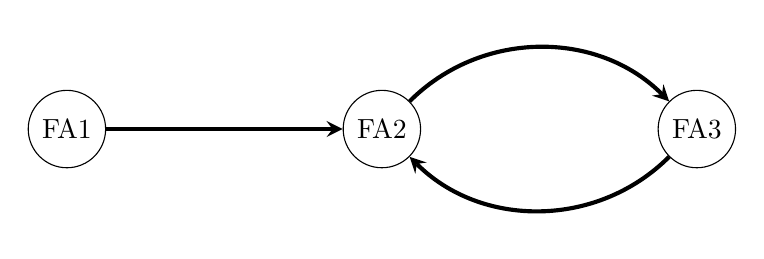
\begin{tikzpicture}
      % Define nodes
      \node[circle, draw] (A) at (0,0) {FA1};
      \node[circle, draw] (B) at (4,0) {FA2};
      \node[circle, draw] (C) at (8,0) {FA3};
      
      % Define edges
      \draw[->, >=stealth, line width=1.5pt] (A) -- (B);
      \draw[->, >=stealth, line width=1.5pt] (B) edge[bend left=45] (C);
      \draw[->, >=stealth, line width=1.5pt] (C) edge[bend left=45] (B);
    \end{tikzpicture}
    \caption{Task Dependencies for First Algorithm Development, self elaborated}
    \label{FA_dependences}
\end{figure}

\section{Second Algorithm Development \textbf{(SA)}}
This is the final section and the goal of this work, here I will try to improve the original algorithm.
Again, here I will only need my personal laptop and access to internet resources.
This section will need a lot of contact with my supervisor and co-supervisor, specially my co-supervisor, who is the expert in the algorithm.
Here the dependence are similar to the previous section (\textbf{see Figure \ref{SA_dependences}}), as is also a development of an algorithm.
This task is especial, because it is difficult to estimate the exact scope of my project, so maybe I make some improvement and then have more time to repeat this process and make another improvement.
\begin{itemize}
    \item \textbf{SA1} Finding Weak Points \\
        Here I will be looking for possible improvements in the code.\\
        Role: Haskell Developer and Researcher\\
        Expected dedication: 15 hours
        \item \textbf{SA2} Improvement Scaffolds \\
        Here will be set the base for the improvements of the algorithms find in the previous task
        Check for possible libraries and codes \\
        Role: Haskell Developer \\
        Expected dedication: 15 hours
    \item \textbf{SA3} Algorithm Implementation\\
        This part is the pure implementation of the algorithm. \\
        Role: Haskell Developer \\
        Expected dedication: 80 hours
    \item \textbf{SA4} Algorithm Testing \\
        Testing of the algorithm implementation, little changes are also contemplated here (no big changes).
        Here more time is needed in comparation of previous section as the size of the code and algorithm\\
        Role: Haskell Developer \\
        Expected dedication: 20 hours
\end{itemize}
\begin{figure}[h]
    \centering
    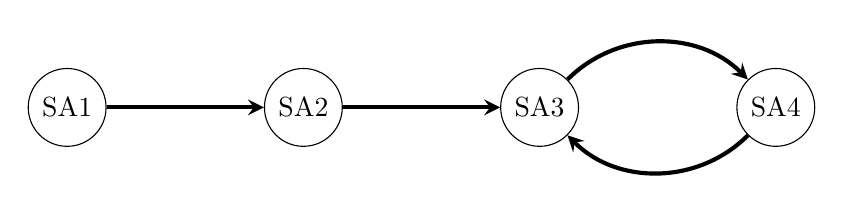
\begin{tikzpicture}
      % Define nodes
      \node[circle, draw] (A) at (0,0) {SA1};
      \node[circle, draw] (B) at (3,0) {SA2};
      \node[circle, draw] (C) at (6,0) {SA3};
      \node[circle, draw] (D) at (9,0) {SA4};
      
      % Define edges
      \draw[->, >=stealth, line width=1.5pt] (A) -- (B);
      \draw[->, >=stealth, line width=1.5pt] (B) -- (C);
      \draw[->, >=stealth, line width=1.5pt] (C) edge[bend left=45] (D);
      \draw[->, >=stealth, line width=1.5pt] (D) edge[bend left=45] (C);
    \end{tikzpicture}
    \caption{Task Dependencies for Second Algorithm Development, self elaborated}
    \label{SA_dependences}
\end{figure}

\section{Documentation \textbf{(D)}}
Finally, this last section is a bit special because it is not planned to be done at the end of the all the previous sections.
It is planned to be done in parallel as the project is developed and the different sections are finished.
Here, all I need is my personal laptop to write all the documentation using \LaTeX.
Here I may need to contact for some help and feedback, but is not mandatory.
There are no direct dependence, but we can consider that we need to complete one section or task before starting to write, so we can consider a graph like shown below (\textbf{see Figure \ref{D_dependences}}).
\begin{itemize}
    \item \textbf{D1} Documentation of RL section \\
        This corresponds to the documentation of the research and learning section. \\
        Role: Project Manager \\
        Expected dedication: 10 hours
    \item \textbf{D2} Documentation of FA section\\
        This corresponds to the documentation of the first algorithm section. \\
        Role: Project Manager \\
        Expected dedication: 20 hours
    \item \textbf{D3} Documentation of SA section \\
        This corresponds to the documentation of the second algorithm section. \\
        Role: Project Manager \\
        Expected dedication: 20 hours
    \item \textbf{D4} Final Documentation \\
    This corresponds to the union of all the previous parts, with the additional parts (conclusions, bibliography, etc.) and the revision of the entire document. \\
    Role: Project Manager \\
    Expected dedication: 50 hours        
\end{itemize}
\begin{figure}[h]
    \centering
    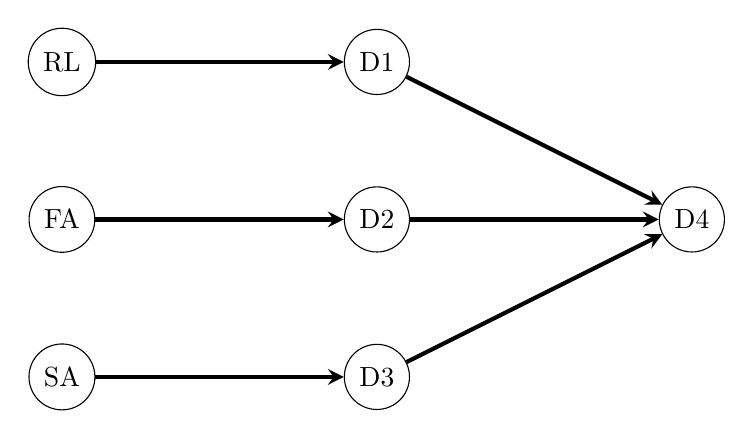
\begin{tikzpicture}
      % Define nodes
      \node[circle, draw] (A) at (4,4) {D1};
      \node[circle, draw] (B) at (4,2) {D2};
      \node[circle, draw] (C) at (4,0) {D3};
      \node[circle, draw] (D) at (8,2) {D4};

      \node[circle, draw] (E) at (0,4) {RL};
      \node[circle, draw] (F) at (0,2) {FA};
      \node[circle, draw] (G) at (0,0) {SA};
      
      % Define edges
      \draw[->, >=stealth, line width=1.5pt] (A) -- (D);
      \draw[->, >=stealth, line width=1.5pt] (B) -- (D);
      \draw[->, >=stealth, line width=1.5pt] (C) -- (D);
      \draw[->, >=stealth, line width=1.5pt] (E) -- (A);
      \draw[->, >=stealth, line width=1.5pt] (F) -- (B);
      \draw[->, >=stealth, line width=1.5pt] (G) -- (C);
    \end{tikzpicture}
    \caption{Task Dependencies for Documentation, self elaborated}
    \label{D_dependences}
\end{figure}

\chapter{Estimations and Gantt chart}
\section{Summary table}
Now that we defined all the tasks, minimum hours and dependence, we can make this following summary table:
\definecolor{LightGray}{rgb}{0.8,0.8,0.8}
\begin{table}[H]
    \begin{adjustwidth}{-1in}{-1in}
    \centering
    \begin{tabular}{|p{5cm}|c|c|p{2cm}|p{3cm}|p{3cm}|}
    \hline
    \textbf{Description} & \textbf{TAG} & \textbf{Hours} & \textbf{Previous Tasks} & \textbf{Requirements} & \textbf{Human Resource} \\
    \hline
    \hline	
    \rowcolor{LightGray}
    \textbf{Project definition and planning} & \textbf{G} & \textbf{75} & \textbf{-} & \textbf{-} & \textbf{-}  \\
    \hline
    Context and Scope & G1 & 20 & Laptop & None & None \\
    \hline
    Planning & G2 & 12 & G1 & Laptop & GEP Tutor \\
    \hline
    Budget and Sustainability & G3 & 18 & G2 & Laptop & GEP Tutor \\
    \hline
    Final Document & G4 & 25 & G3 & Laptop & GEP Tutor \\
    \hline
    \hline
    \rowcolor{LightGray}
    \textbf{Research and Learning} & \textbf{RL} & \textbf{75} & \textbf{G} & \textbf{-} & \textbf{-} \\
    \hline
    Haskell Refresh & RL1 & 20 & None & Laptop, Books & Supervisor \\
    \hline
    TFM assimilation & RL2 & 25 & None & Laptop & Supervisors \\
    \hline
    Dynamic Pipeline Framework & RL3 & 30 & RL1, RL2 & Laptop & Juan Pablo \\
    \hline
    \hline
    \rowcolor{LightGray}
    \textbf{First Algorithm Development} & \textbf{FA} & \textbf{80} & \textbf{RL} & \textbf{-} & \textbf{-} \\
    \hline
    Algortim Scaffold & FA1 & 20 & None & None & Supervisors\\
    \hline
    Algorith Implementation & FA2 & 50 & FA1 & Laptop & Supervisor\\
    \hline
    Algorithm Testing & FA3 & 10 & FA2 & Laptop & None \\
    \hline
    \hline
    \rowcolor{LightGray}
    \textbf{Second Algorithm Development} & \textbf{SA} & \textbf{130} & \textbf{FA} & \textbf{-} & \textbf{-} \\
    \hline
    Finding Weak Points & SA1 & 15 & None & Laptop & Co-supervisor\\
    \hline
    Improvement Scaffolds & SA2 & 15 & SA1 & None & None\\
    \hline
    Algorith Implementation & SA3 & 80 & SA2 & Laptop & Supervisor\\
    \hline
    Algorithm Testing & SA4 & 20 & SA3 & Laptop & None\\
    \hline
    \hline
    \rowcolor{LightGray}
    \textbf{Documentation} & \textbf{D} & \textbf{100} & \textbf{RL,FA,SA,G} & \textbf{-} & \textbf{-} \\
    \hline
    Documentation of RL section & D1 & 10 & RL & Laptop & None \\
    \hline
    Documentation of FA section & D2 & 20 & FA & Laptop & None \\
    \hline
    Documentation of SA section & D3 & 20 & SA & Laptop & None \\
    \hline
    Final Documentation & D4 & 50 & D1, D2, D3 & Laptop & Supervisors \\
    \hline
    \hline
    \rowcolor{LightGray}
    \multicolumn{6}{|c|}{\textbf{Total (G + RL + FA + SA + D): 460 hours}}  \\
    \hline
    \end{tabular}
    \caption{Summary of Project Planning, self elaborated}
    \label{TableResume}
    \end{adjustwidth}
\end{table}
\section{Gantt chart}

\definecolor{G_Color}{rgb}{1,0,0}
\definecolor{RL_Color}{rgb}{0,1,0}
\definecolor{FA_Color}{rgb}{0,0,1}
\definecolor{SA_Color}{rgb}{1,1,0}
\definecolor{D_Color}{rgb}{0,1,1}

\begin{figure}[H]
    \begin{adjustwidth}{-1in}{-1in}
    \centering
    \begin{ganttchart}[vgrid, hgrid, x unit=0.55cm, y unit chart=0.6cm]{1}{17}
    \gantttitle{Week}{17} \\
    \gantttitlelist{1,...,17}{1} \\
    %SECTION G
    \ganttgroup{G - Project definition and planning [75]}{1}{4} \\ 
    \ganttbar[bar/.style={draw=black, fill=G_Color}] {G1 - Context and Scope [20h]}{1}{1} \\
    \ganttbar[bar/.style={draw=black, fill=G_Color}] {G2 - Planning [12h]}{2}{2} \\
    \ganttbar[bar/.style={draw=black, fill=G_Color}] {G3 - Budget and Sustainability [18h]}{3}{3} \\
    \ganttbar[bar/.style={draw=black, fill=G_Color}] {G4 - Final Document [25h]}{4}{4} \\
    \ganttlink{elem1}{elem2}
    \ganttlink{elem2}{elem3}
    \ganttlink{elem3}{elem4}

    %SECTION RL
    \ganttgroup{RL - Research and Learningt [75]}{5}{7} \\ 
    \ganttbar[bar/.style={draw=black, fill=RL_Color}] {RL1 - Haskell Refresh [20h]}{5}{5} \\
    \ganttbar[bar/.style={draw=black, fill=RL_Color}] {RL2 - TFM assimilation [25h]}{6}{6} \\
    \ganttbar[bar/.style={draw=black, fill=RL_Color}] {RL3 - Dynamic Pipeline Framework [30h]}{7}{7} \\
    \ganttlink{elem0}{elem5}
    \ganttlink{elem6}{elem8}
    \ganttlink{elem7}{elem8}

    %SECTION FA
    \ganttgroup{FA - First Algorithm Development [80]}{8}{10} \\ 
    \ganttbar[bar/.style={draw=black, fill=FA_Color}] {FA1 - Algortim Scaffold [20h]}{8}{8} \\
    \ganttbar[bar/.style={draw=black, fill=FA_Color}] {FA2 - Algorith Implementation [50h]}{9}{10} \\
    \ganttbar[bar/.style={draw=black, fill=FA_Color}] {FA3 - Algorithm Testing [10h]}{10}{10} \\
    \ganttlink{elem5}{elem9}
    \ganttlink{elem10}{elem11}
    \ganttlink{elem11}{elem12}

    %SECTION SA
    \ganttgroup{FA - Second Algorithm Development [130]}{11}{15} \\ 
    \ganttbar[bar/.style={draw=black, fill=SA_Color}] {SA1 - Finding Weak Points [15h]}{11}{11} \\
    \ganttbar[bar/.style={draw=black, fill=SA_Color}] {SA2 - Improvement Scaffolds [15h]}{12}{12} \\
    \ganttbar[bar/.style={draw=black, fill=SA_Color}] {SA3 - Algorith Implementation [80h]}{12}{15} \\
    \ganttbar[bar/.style={draw=black, fill=SA_Color}] {SA4 - Algorithm Testing [20h]}{15}{15} \\
    \ganttlink{elem9}{elem13}
    \ganttlink{elem14}{elem15}
    \ganttlink{elem15}{elem16}
    \ganttlink{elem16}{elem17}
    %SECTION D
    \ganttgroup{D - Documentation [100]}{8}{17} \\
    \ganttbar[bar/.style={draw=black, fill=D_Color}] {D1 - Documentation of RL section [10h]}{8}{10} \\
    \ganttbar[bar/.style={draw=black, fill=D_Color}] {D2 - Documentation of FA section [20h]}{11}{15} \\
    \ganttbar[bar/.style={draw=black, fill=D_Color}] {D3 - Documentation of SA section [20h]}{16}{16} \\
    \ganttbar[bar/.style={draw=black, fill=D_Color}] {D4 - Final Documentation [50h]}{16}{17} \\

    \ganttlink{elem5}{elem19}
    \ganttlink{elem9}{elem20}
    \ganttlink{elem13}{elem21}
    \ganttlink{elem19}{elem22}
    \ganttlink{elem20}{elem22}
    \ganttlink{elem21}{elem22}
    
    \label{GANTT}
    \end{ganttchart}
    \caption{Gantt Diagram of this project, self elaborated}
    \end{adjustwidth}
\end{figure}

\chapter{Risk management: obstacles and alternatives}
As mentioned in previous sections of this work, there are some potential risks that may appear during the development of the project.
Here will be explained how I will manage them and the alternatives that could be done in case of critical obstacles.
\section{Obstacles}
\subsection*{Time deadline}
As said previously, this is one of the most important risks of the project. There is not a lot of time, but I have some tools to deal with this problem.
Firstly, the main objective is to obtain more time if needed and my principal activity (and the one that spends more time) is my job as intern.
I have flexibility in my schedule and I can reorganize my week to spend more time in the project.
Also, I have some holidays that I can use to spend more time in the project.
\subsection*{Dynamic Pipeline Framework}
I explained that I never used before this framework and I may have some problems with it or it could have some bugs or limitations.
The principal tool to deal with is to contact with his creator, Juan Pablo. Also, I can spend more time studying the framework because I saved some time in case of this obstacle.
This problem could potentially add from 10 to 30 hours to the project.
\section{Alternatives}
If some of the previous obstacles appear and I can not deal with them, I could be forced to make some changes in the project.
So the principal alternative is to reduce the scope of the project, reducing the time spent in the last section: the improvement of the algorithm.
This part is the longest of the project and it is planned to be able to be reduced if needed.
It is very comfortable, since I do not need any additional resource and I can adapt it to the time that I have left.
